% This is "www2008-sample.tex" copied from "www2005-sample.tex" V1.2 January 26 2004
% This file should be compiled with V1.4 of "www2008-submission.class"
%
% This example file demonstrates the use of the 'www2008-submission.cls'
% V1.4 LaTeX2e document class file. It is for those submitting
% articles to the WWW'04 Conference WHO DO NOT WISH TO 
% STRICTLY ADHERE TO THE SIGS (PUBS-BOARD-ENDORSED) STYLE.
% The 'www2008-submission.cls' file will produce a similar-looking,
% albeit, 'tighter' paper resulting in, invariably, fewer pages.
%
% ----------------------------------------------------------------------------------------------------------------
% This .tex file (and associated .cls V1.4) produces:
%       1) NO Permission Statement
%       2) WWW'04-specific conference (location) information
%       3) The Copyright Line with ACM data
%       4) NO page numbers
%
% ---------------------------------------------------------------------------------------------------------------
% This .tex source is an example which *does* use
% the .bib file (from which the .bbl file % is produced).
% REMEMBER HOWEVER: After having produced the .bbl file,
% and prior to final submission, you *NEED* to 'insert'
% your .bbl file into your source .tex file so as to provide
% ONE 'self-contained' source file.
%
% ================= IF YOU HAVE QUESTIONS =======================
% Questions regarding the SIGS styles, SIGS policies and
% procedures, Conferences etc. should be sent to
% Julie Goetz (goetz@acm.org) or Adrienne Griscti (griscti@acm.org)
%
% Technical questions only to
% Gerald Murray (murray@acm.org)
% ===============================================================
%
% For tracking purposes - this is V1.2 - January 26 2004
\documentclass{../templates/www2008-submission}

% shared affiliation macro
\def\sharedaffiliation{
\end{tabular}
\begin{tabular}{c}}

\begin{document}
%
\title{Bootstrapping the Semantic Web of Social Online Communities}
%\subtitle{[Extended Abstract]
%\titlenote{A full version of this paper is available as
%\textit{Author's Guide to Preparing ACM SIG Proceedings Using
%\LaTeX$2_\epsilon$\ and BibTeX} at
%\texttt{www.acm.org/eaddress.htm}}}
%
% You need the command \numberofauthors to handle the "boxing"
% and alignment of the authors under the title, and to add
% a section for authors number 4 through n.
%
% Up to the first three authors are aligned under the title;
% use the \alignauthor commands below to handle those names
% and affiliations. Add names, affiliations, addresses for
% additional authors as the argument to \additionalauthors;
% these will be set for you without further effort on your
% part as the last section in the body of your article BEFORE
% References or any Appendices.

\numberofauthors{3}
%
% Put no more than the first THREE authors in the \author command

% NOTE: All authors should be on the first page. For instructions
% for more than 3 authors, see:
% http://www.acm.org/sigs/pubs/proceed/sigfaq.htm#a18

%		\author{
%
% The command \alignauthor (no curly braces needed) should
% precede each author name, affiliation/snail-mail address and
% e-mail address. Additionally, tag each line of
% affiliation/address with \affaddr, and tag the
%% e-mail address with \email.

%\alignauthor Diego Berrueta\\
%       \affaddr{Fundaci\'on CTIC}\\
%       \affaddr{Gij\'on, Asturias, Spain}
%\and
%\alignauthor Sergio Fern\'andez\\
%       \affaddr{Fundaci\'on CTIC}\\
%       \affaddr{Gij\'on, Asturias, Spain}\\
%       \email{\{fname.surname\}@fundacionctic.org}
%\and
%\alignauthor Lian Shi\\
%       \affaddr{Fundaci\'on CTIC}\\
%       \affaddr{Gij\'on, Asturias, Spain}
%}

\author{
  \alignauthor Diego Berrueta \\
%  \email{diego.berrueta@fundacionctic.org}
%
  \alignauthor Sergio Fern\'andez \\
%  \email{sergio.fernandez@fundacionctic.org}
%
  \alignauthor Lian Shi \\
%  \email{lian.shi@fundacionctic.org}
%
  \sharedaffiliation
    %\email{\{diego.berrueta,sergio.fernandez,lian.shi\}@fundacionctic.org}
    \affaddr{\{diego.berrueta,sergio.fernandez,lian.shi\}@fundacionctic.org} \\
    \affaddr{R\&D Department, Fundaci\'on CTIC}  \\
    \affaddr{Gij\'on, Asturias, Spain}
}

%\additionalauthors{Additional authors: John Smith (The Th{\o}rv\"{a}ld Group,
%email: {\texttt{jsmith@affiliation.org}}) and Julius P.~Kumquat
%(The Kumquat Consortium, email: {\texttt{jpkumquat@consortium.net}}).}

%\date{5 February 2008}

\maketitle

\begin{abstract}
Mining and searching the social web is hardly possible without
a significative amount of data available in an interoperable
format. This paper enumerates and compares several techniques which can be
applied to produce large quantities of RDF data describing
social web sites. Advantages, drawbacks and potential issues of
each of these techniques are discussed. Practical applications
are presented to illustrate the convenience of each approach.
\end{abstract}

% A category with only the three required fields
%\category{H.4.m}{Information Systems}{Miscellaneous}
%\category{D.2}{Software}{Software Engineering}
%A category including the fourth, optional field follows...
%\category{D.2.8}{Software Engineering}{Metrics}[complexity measures,
%performance measures]

\keywords{semantic mining, online community, mailing list, rdf, xsl, sioc}

%%%%%%%%%%%%%%%%%%%%%%%%%%%%%%%%%%%%%%%%%%%%%%%%%%%%%%%%%%%%
\section{Introduction}

Effective large-scale mining of the social web requires the
availability of a significative amount of well-defined data.
The semantic web provides a convenient platform to publish and
consume these data. There are a couple of vocabularies (FOAF~\cite{FOAF} and
SIOC~\cite{Bojars2007}) that are particularly suited to represent the
information of the social web using an interoperable formalism.
However, so far only a small portion of the social web is
represented in these vocabularies.

In this paper we survey and classify a number of techniques that
are targeted to create semantic web enabled representations of
the information of the social web. We focus on online communities
and discussion forums, although these techniques remain valid
for other social web sites. The combination of all these
techniques can provide enough momentum to the semantic social
web and it can help to reach the critical-mass that
enables a virtuous cycle of applications and data.

The rest of the paper is organized as follows: (FIXME).

%%%%%%%%%%%%%%%%%%%%%%%%%%%%%%%%%%%%%%%%%%%%%%%%%%%%%%%%%%%%
\section{Technologies}

We use an ontology and RDF (Resource Description
Framework~\cite{RDF}) to publish online communities into 
the (Semantic) Web, while retaining the meta-data that were present in 
the messages. Additionally, by doing so, the information can be
merged and linked to other vocabularies, such as FOAF.

DERI Galway leads the development of SIOC (Semantically-Interlinked Online
Communities\footnote{\url{http://sioc-project.org/}}), an ontology that 
provides a vocabulary to interconnect different discussion methods such 
as blogs, web-based forums and mailing lists~\cite{Breslin2006,Breslin2005}.
SIOC is now an official W3C member submission~\cite{Bojars2007}.
SIOC has been used as the core framework to represent information from
online communities in all the work described in this paper.

\begin{figure}[ht]
 \centering
 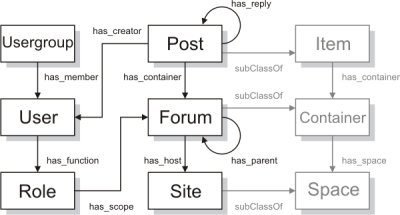
\includegraphics[width=7cm]{images/sioc.png}
 \caption{SIOC main classes and properties}
\end{figure}

%%%%%%%%%%%%%%%%%%%%%%%%%%%%%%%%%%%%%%%%%%%%%%%%%%%%%%%%%%%%
\section{Classification of SIOC-producing techiques}

Since SIOC is a recent specification, its adoption is still low, and
only a few sites export SIOC data. There are a number of techniques
that can be used to bootstrap a network of semantic descriptions from
current social sites. We classify them in two categories:

\begin{itemize}
\item Those which require direct access to the underlying database behind
the social web site are \emph{intrusive techniques}.
\item On the other hand, techniques which do not require direct access to
the database and can operate on resources already published on the web
are \emph{non-intrusive}.
\end{itemize}

We further describe each category in the following paragraphs.

\subsection{Intrusive techniques}

It is safe to say that every social web site is built on top of a
database that serves as the information model. The web application
acts as the controller and publishes different views of the model in
formats such as HTML and RSS. In terms of this pattern, publishing
SIOC data is as simple as adding a new view.
From a functional point of view, this is the most powerful scenario, because
it allows a loseless publication due to the direct access
to the backend database.

The SIOC community is contributing a number of plug-ins for some
popular web community applications, such as Drupal, WordPress and 
PhpBB\footnote{A more complete and up-to-date list is available
at \url{http://sioc-project.org/exporters}.}. Mailing lists are
also covered by SWAML, which will be discussed below.

There is, however, a major blocker for this approach. All these
software components need a deployment in the server side (where
the database is). This is a burden for system administrators, who
are often unwilling to make a move that would make it more difficult to
maintain, securize and upgrade their systems. This is particularly
true when there is no obvious inmmediate benefit of exporting
SIOC data (\emph{chicken-and-egg} problem).

\subsection{Unintrusive techniques}

In absence of direct access to the database, unintrusive
techniques exploit the information already available on the web:

\begin{itemize}

\item Cooked HTML views of the information, the same ones that
are rendered by web browsers for human consumption.
Even if this source is always available,
its exploitation poses a number of issues described in Section~FIXME.

\item RSS/Atom feeds, which have become very popular. They can be easily
translated into RDF data using XSLT stylesheets (for XML-based feeds) or SPARQL queries\footnote{\url{http://apassant.net/blog/2006/10/05/from-rss-to-sioc-using-sparql/}}
(for RSS 1.0, which is actually RDF). Unfortunately,
these feeds often contain just partial descriptions.

\item Public APIs. The web~2.0 trend has pushed some social web
sites to export (part of) their functionality through APIs
to enable their consumption by third-party mash-ups and applications.
Where available, these APIs offer an excellent opportunity to
create RDF views of the data.

\end{itemize}

A shared aspects of these sources is their ubiquous availability through
web protocols and languages, such as HTTP and XML. Therefore, they
can be consumed anywhere, thus freeing the system administrators of
taking care of any additional deployment. In contrast, they cannot compete
with the intrusive approaches in terms of information quality, as
any access to the data is not primary.

%%%%%%%%%%%%%%%%%%%%%%%%%%%%%%%%%%%%%%%%%%%%%%%%%%%%%%%%%%%%
\section{Case studies}

In this section we describe an example of each of the two approaches
aforementioned.

\subsection{From mboxes to RDF: SWAML}

SWAML~\cite{SWAML2007} is a Python script that reads mailing 
list archives in raw format, typically stored in a ``mailbox'' 
(or ``mbox''), as defined in RFC~4155~\cite{RFC4155}. It parses
mailboxes and outputs RDF descriptions of the messages, mailing lists
and users as instances of the SIOC ontology. Internally, it re-constructs
the structure of the conversations in a tree structure, and it exploits
this structure to produce links between the posts.

This script is highly configurable and non-interactive, and has been
designed to be invoked by the system task scheduler. This low-coupling with
the software that runs the mailing list eases its portability and
deployment.

SWAML is classified as an example of the intrusive techniques because
it actually requires access to the primary data source, even if
it is not a relational database but a text file. Anyway, it is
worth mention that some servers already export these text files
(mailboxes) through HTTP. Therefore, sometimes it is possible to
retrieve the mailbox and build a perfect replica of the primary
database in another box. This enables to use SWAML without the
participation of the system administration of the original
web server.

\subsection{Scraping HTML by means of XSLT}

Web scraping is a well-known, non-intrusive and widely used technique,
although it should be applied only when other approaches are not viable.
Screen-scraping applications are difficult to maintain and
often produce low-quality information.

A popular language to write HTML scrapers is XSLT. As a pre-requisite,
the mark-up must be converted to XHTML (an XML dialect) if it is not
already in this format. Fortunately, open source utilities such as
Tidy\footnote{\url{http://tidy.sourceforge.net/}} do a decent job
to clean and fix HTML files with a poor mark-up.

Scraping functions are often tied to a web crawler to follow the
links between HTML pages.

As each web site uses a different, customized template to
publish their cooked HTML files, it is
difficult to develop a generic scraper, even for a single social
web application. Moreover, there are lots of different social and
web-community applications, and thus the portability of scrapers
is very low.

The output of a web scraper implemented in XSLT can be RDF/XML, but
another interesting posibility has already been explored. In
mle~\cite{Hausenblas2007}, the authors use XSLT to decorate the
DOM tree of an XHTML page with RDFa attributes~(FIXME: cite RDFa).
This creates an hybrid representation which is readable for
humans \emph{and} semantic web agents.


%%%%%%%%%%%%%%%%%%%%%%%%%%%%%%%%%%%%%%%%%%%%%%%%%%%%%%%%%%%%
\section{Common problems}

These approaches for mining online communities have some common problem:

\begin{itemize}
  \item \textbf{Identities:} as it can be seen in figure~\ref{fig:foaf-sioc},
	a person (an instance of \texttt{foaf:Person}) can own many online 
	accounts (instances of \texttt{sioc:User}). 

	\begin{figure}[ht]
	 \centering
	 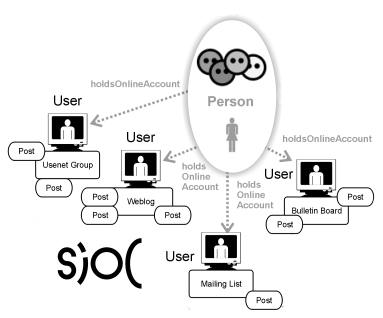
\includegraphics[width=7cm]{images/foaf-sioc.png}
	 \caption{\label{fig:foaf-sioc}Online identity, relationship between FOAF and SIOC}
	\end{figure}

	So we must apply techniques (such as 
	Smushing\footnote{\url{http://esw.w3.org/topic/RdfSmushin}g})
	in order to extract the real identy behind a online account.

  \item \textbf{Problems with sha1 algorithm:} related with previous problem,
	we detected a problem using sha1 algorithm~\cite{Eastlake2001}. FOAF 
	and SIOC use this algorithm (in properties \texttt{foaf:mbox\_sha1sum} 
	and \texttt{sioc:email\_sha1}, respectively) in order to protect email 
	addresses from SPAM attacks. And this algoritm is case sensitive. So,
	for example, if we take Diego's email address, we could write it as
	\texttt{diego.berrueta@fundacionctic.org} or as \texttt{Diego.Berrueta@fundacionctic.org}.
	Both are valid email addresses. But each one generates different sha1sum.
	This could  seem a detail without importance, but it really creates a 
	serious problem when try to identify persons/users using these
	inverse functional properties. Unfortunately in our experimientos we 
	have found many times this kind of problem.

  \item \textbf{\textit{Flat} thread:} Typical structure of Web discussion
	forum is flat: it's imposible to know which post is the parent of
	other. So exporters of this kind of forums (server-side or scrapers)
	create flat thread (\texttt{sioc:Thread}) where all posts always answer
	the first one. This is a very poor information about thread, but it's
	implicit in the anarchic nature of Web forums.

  \item \textbf{Repeated keys:} This problem doesn't exist when there is a 
	central application (such as a Web CMS) that assigns unique identifier 
	for each message posted. But in a mailing list, although each mail 
	message has a supposedly unique identifier in its header 
	(\texttt{Message-ID}, defined by RFC~2822~\cite{RFC2822}), 
	in practice its uniqueness cannot be taken for granted,
	probably due to non-RFC compliant mail transport agents.

  \item \textbf{Paginated discussions:} in scraping approaches, we must be able 
	to process the page in order not to lose important information.

\end{itemize}


%%%%%%%%%%%%%%%%%%%%%%%%%%%%%%%%%%%%%%%%%%%%%%%%%%%%%%%%%%%%
\section{Experimentation with Free\\ Sofware communities}

In order to test and improve our experimentes, we needed social
online communities with coarse amounts of information published.
And we selected Free Software communities, becuase there are a very
open kind of communities. More specifically chose four sites where
test our experiments: GNOME mailing lists, Debian mailing lists,
Ubuntu Forums and Advogato.

\subsection{\label{sec:gnome}GNOME mailing lists}

GNOME project publishes archives of its mailing lists~\footnote{\url{http://mail.gnome.org/archives/}}.
It is an archive with around 200 mailing list with information of 
more than ten years of activity in the project. Fortunately these
archives are not only published in (X)HTML, but also there are 
available (gzipped) mailboxes for each month. So we wrotte a simple
crawler to fetch these raw data directly by HTTP, and merge archive
of each month in a single mailbox for each mailing list of the project.

Then we had all necessary information to start running SWAML on these 
more than 200 mailboxes. For a selected subset of the mailing lists, 
SWAML has produced plus 25 million triples.

\subsection{Debian mailing lists}

FIXME

Using these approach we have collected \textbf{FIXME} RDF triples
from a selected subset of \textbf{FIXME: number of lists} lists for
the period 2005-2006.

\subsection{Ubuntu Forums}

Ubuntu Forums\footnote{\url{http://ubuntuforums.org/}} are a very popular 
discussion forusm among users of this GNU/Linux distribution. They have a 
frenetic activity, with plus than 4 million of posts in the moment we made
our experiments.

In these forums we used a quite similar appoach than with Debian mailing
lists. We analized the markup generated by vBulletin (CMS used in these forums)
and we developed some XSLT stylesheets to transform get instances of
\texttt{sioc:Forum}, \texttt{sioc:Thread} and \texttt{sioc:Post}. We 
selected only a subset of available forums to test our application, FIXME

\subsection{Advogato}

FIXME


%%%%%%%%%%%%%%%%%%%%%%%%%%%%%%%%%%%%%%%%%%%%%%%%%%%%%%%%%%%%
\section{\label{sec:conclusions}Conclusions}

Semantic descriptions of online communities pushes them
into a new level of functionality. On the one hand, they can be
conveniently browsed and queried. Search engines can exploit the
metadata to improve their precission, and at the same time, to
avoid repeated results.

On the other hand, the semantic descriptions can be
analysed and mined. Futhermore, they can be linked to other resources,
thus reducing the risk of creating an ``information silo'' and
enabling the rise of a network of ``linked data''.

So far, no semantic annotation relative to the meaning of
the messages is considered. Obviously, it is very difficult
to extract such information from the message text.
However, it is conceivable that it can be added by other 
means, such as social tagging using folksonomies, or parsing the 
RDFa that may exist in the e-mail messages that are send in XHTML 
format.The inherent community-based nature of mailing lists can
be exploited to build recommendation systems~\cite{Celma2006}.

FIXME

%%%%%%%%%%%%%%%%%%%%%%%%%%%%%%%%%%%%%%%%%%%%%%%%%%%%%%%%%%%%
\section*{Acknowledgements}

FIXME


% The following two commands are all you need in the
% initial runs of your .tex file to
% produce the bibliography for the citations in your paper.
\bibliographystyle{abbrv}
\bibliography{../references}

\balancecolumns

\end{document}
